\section{\Gls{galapagos assembler}}

The \Gls{galapagos assembler} is an assembler for \Gls{galapagos} Assembly that was written for this project.
It assembles Galapagos assembly to be run on the programmable fitness cores of the Barricelli computer.
The assembler is written in Python. 
It is designed with a modular, object-oriented software architecture, which makes it easily extensible and modifiable.
Indeed, during the short time it has been published on the Internet, it has already been forked and adapted for use for other instruction set architectures and assembly languages.
The assembler supports the entire \Gls{galapagos} instruction set.

With a an assembler available, opportunities for performance optimizations through instruction re-ordering are made available.
The idea is that instructions within a simple code block, i.e. a branch-less block of consecutive instructions with no labels, instructions may be carefully re-ordered to minimize data hazards.
The assembler does not perform these instruction re-orderings.
This is because the forwarding unit in the processor architecture already resolves many of the same issues that the assembler would work around using instruction re-ordering.

The only non-control related hazards that the forwarding unit doesn't already resolve are use-after-load conflicts.
A use-after-load conflict is a conflict where the processor plans the execute a data load from memory, and then use the result from that load in the immediately proceeding execution.
When this happens, the result from the memory load is not yet ready when the execution is planned to execute.
This hazard is resolved off-line by the assembler.
It can detect use-after-load hazards during assembly, and will insert a \gls{nop} between the load and use instructions, forcing the processor to wait until the data is available.

\Gls{galapagos assembler} is available in PyPi, the leading python package index.
This means that it is easily installable for end users using \texttt{pip}, the python package manager.
Installation is as simple as running \texttt{pip install galapagos-assembler} in a terminal where pip is available.

The source code of the \Gls{galapagos assembler} can be found in appendix \vref{appendix:galapagos-assembler-source-code}.

\section{Case}

\begin{figure}[H]
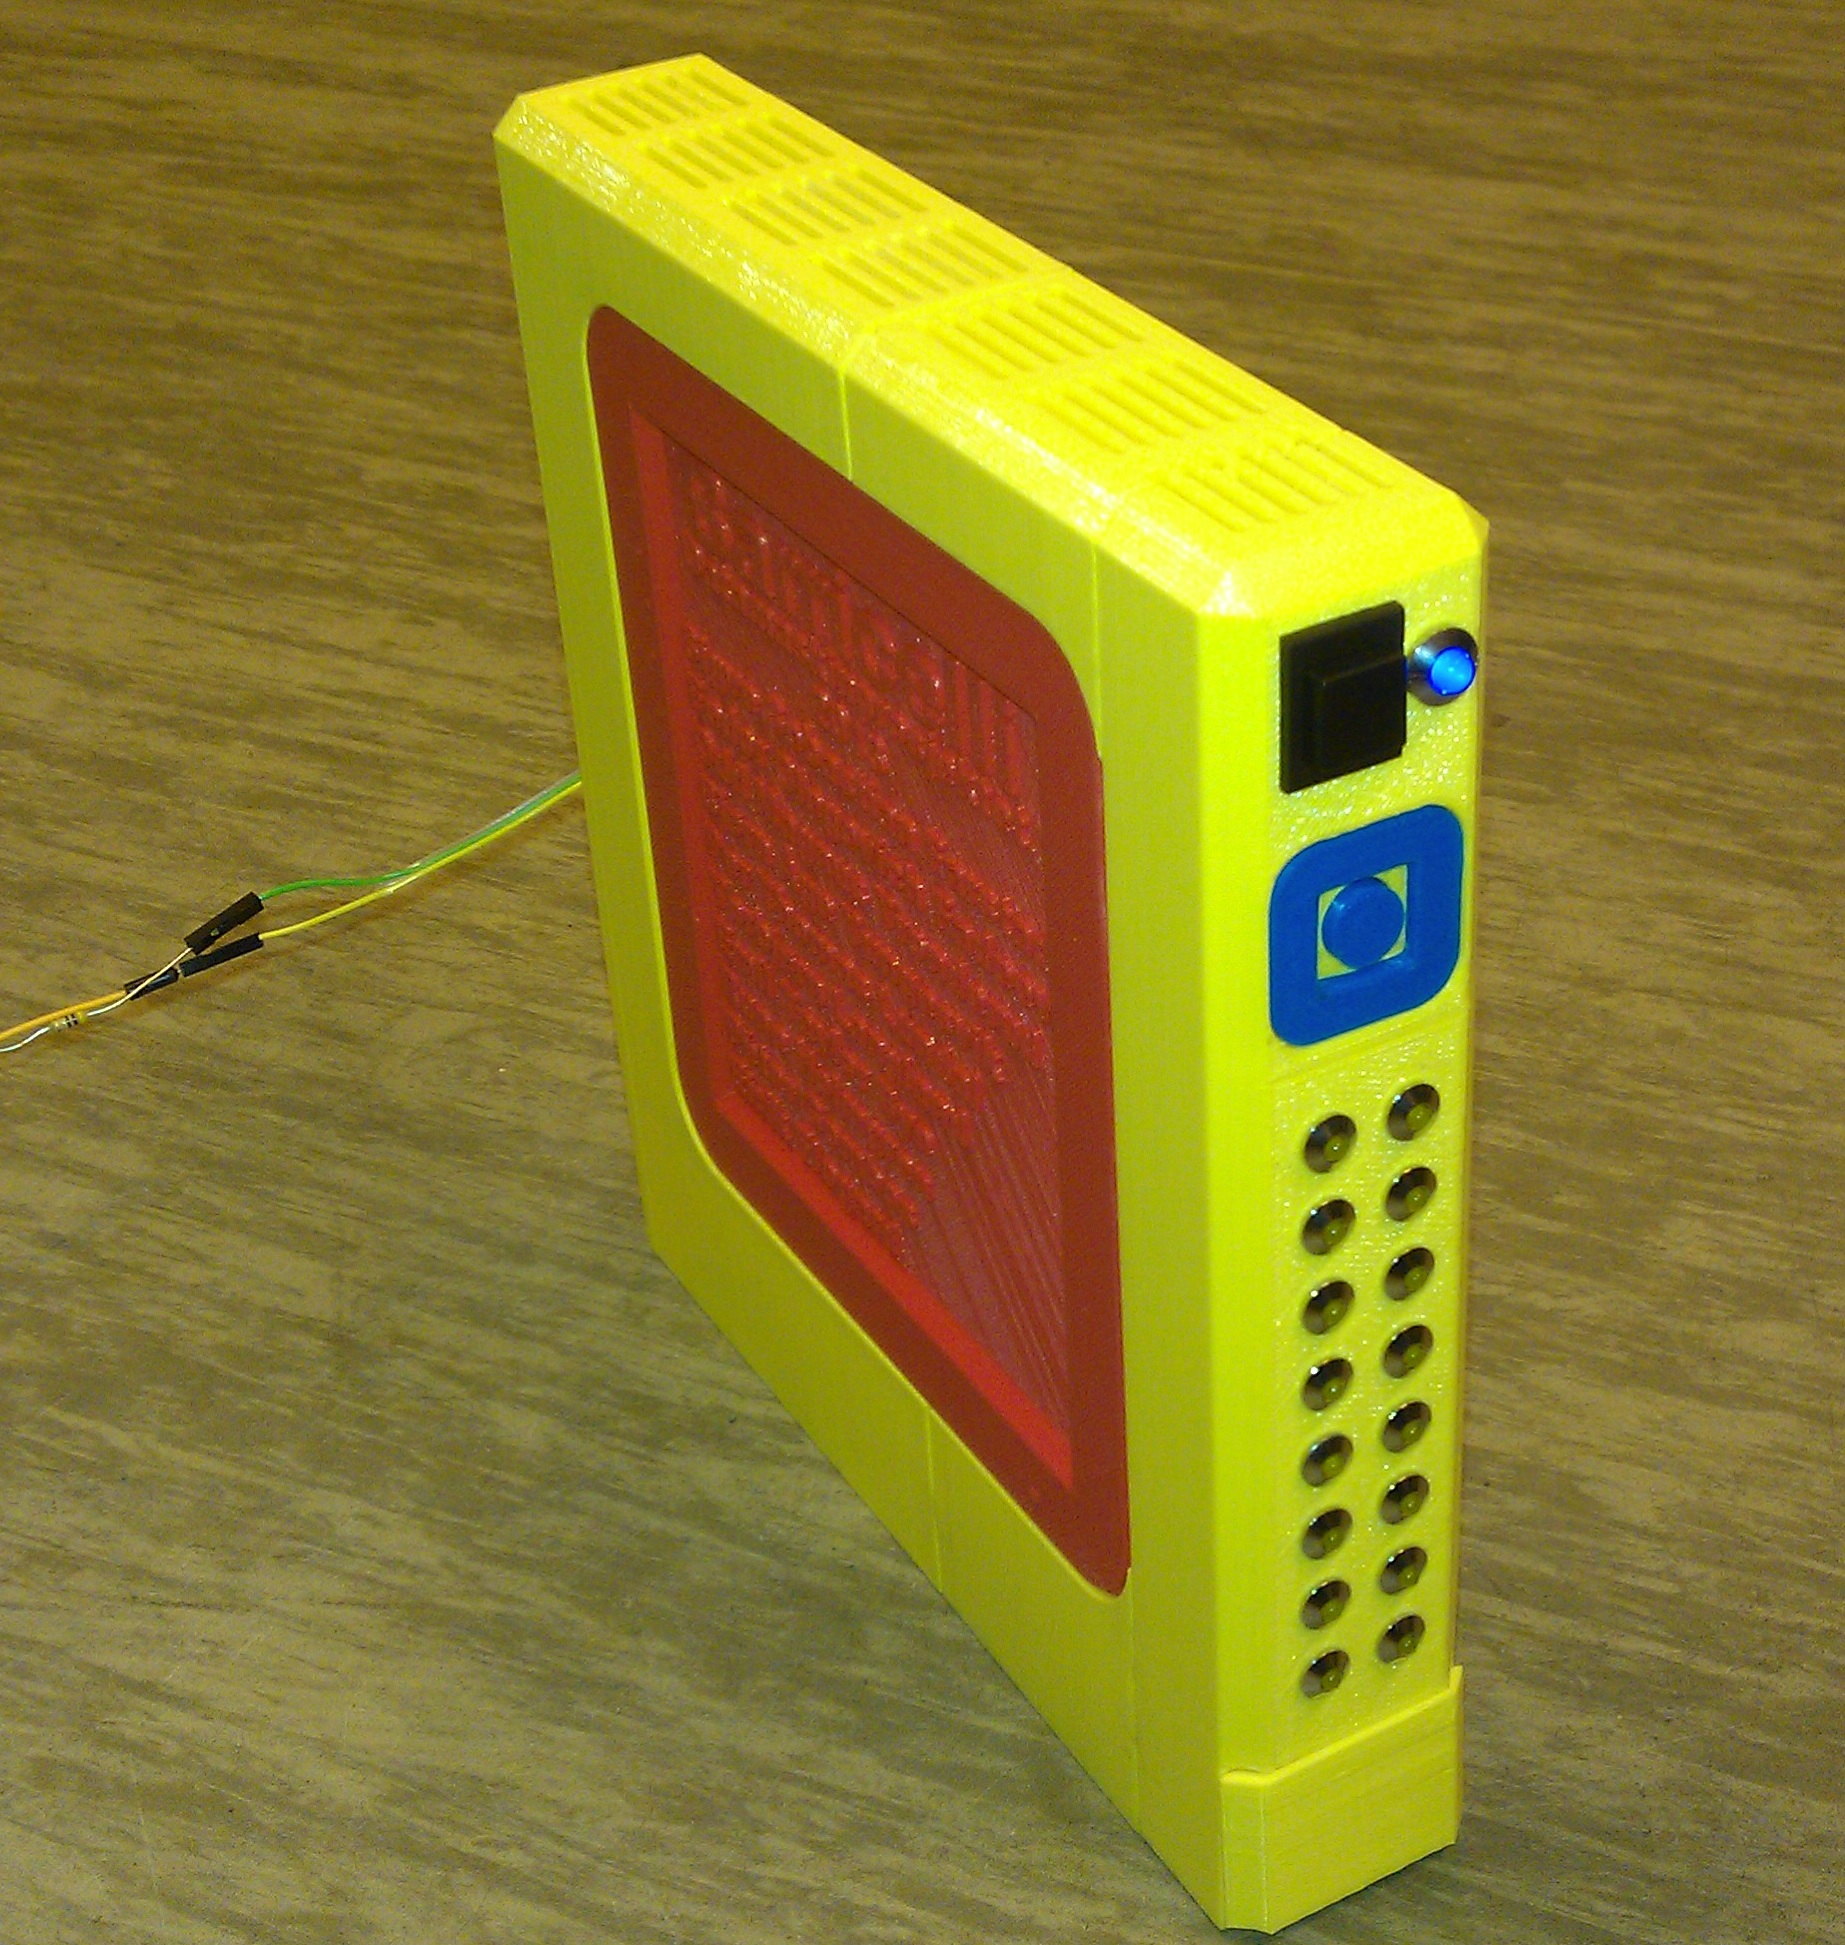
\includegraphics[width=\textwidth,keepaspectratio,clip]{additional-components/case.jpg}%
\caption{Case}
\end{figure}

To give this project a nice presentable finish and professional appearance, the group decided to make a case for the computer.
This was also a good opportunity to develop our skills with 3D modeling.
Because of this we chose to create the case using a 3D printer.

\subsection {Design}

It was early decided that the case should have all of the features of the real board.
This would ensure that the user would be able to operate the computer without ever feeling the need to take the board out of the case.
This is why the case have all of the user controlled LEDs and buttons from the PCB on the case itself, and the buttons and LEDs are available from the board from headers.
The 16 LEDs are placed on the front panel, while the buttons are placed on a small keyboard that slide out on a drawer in front of the case.
The keyboard drawer is loaded by a rubber band that keep it shut, while the mechanism shown here will keep it open when the user have pulled it out.

\begin{figure}[H]
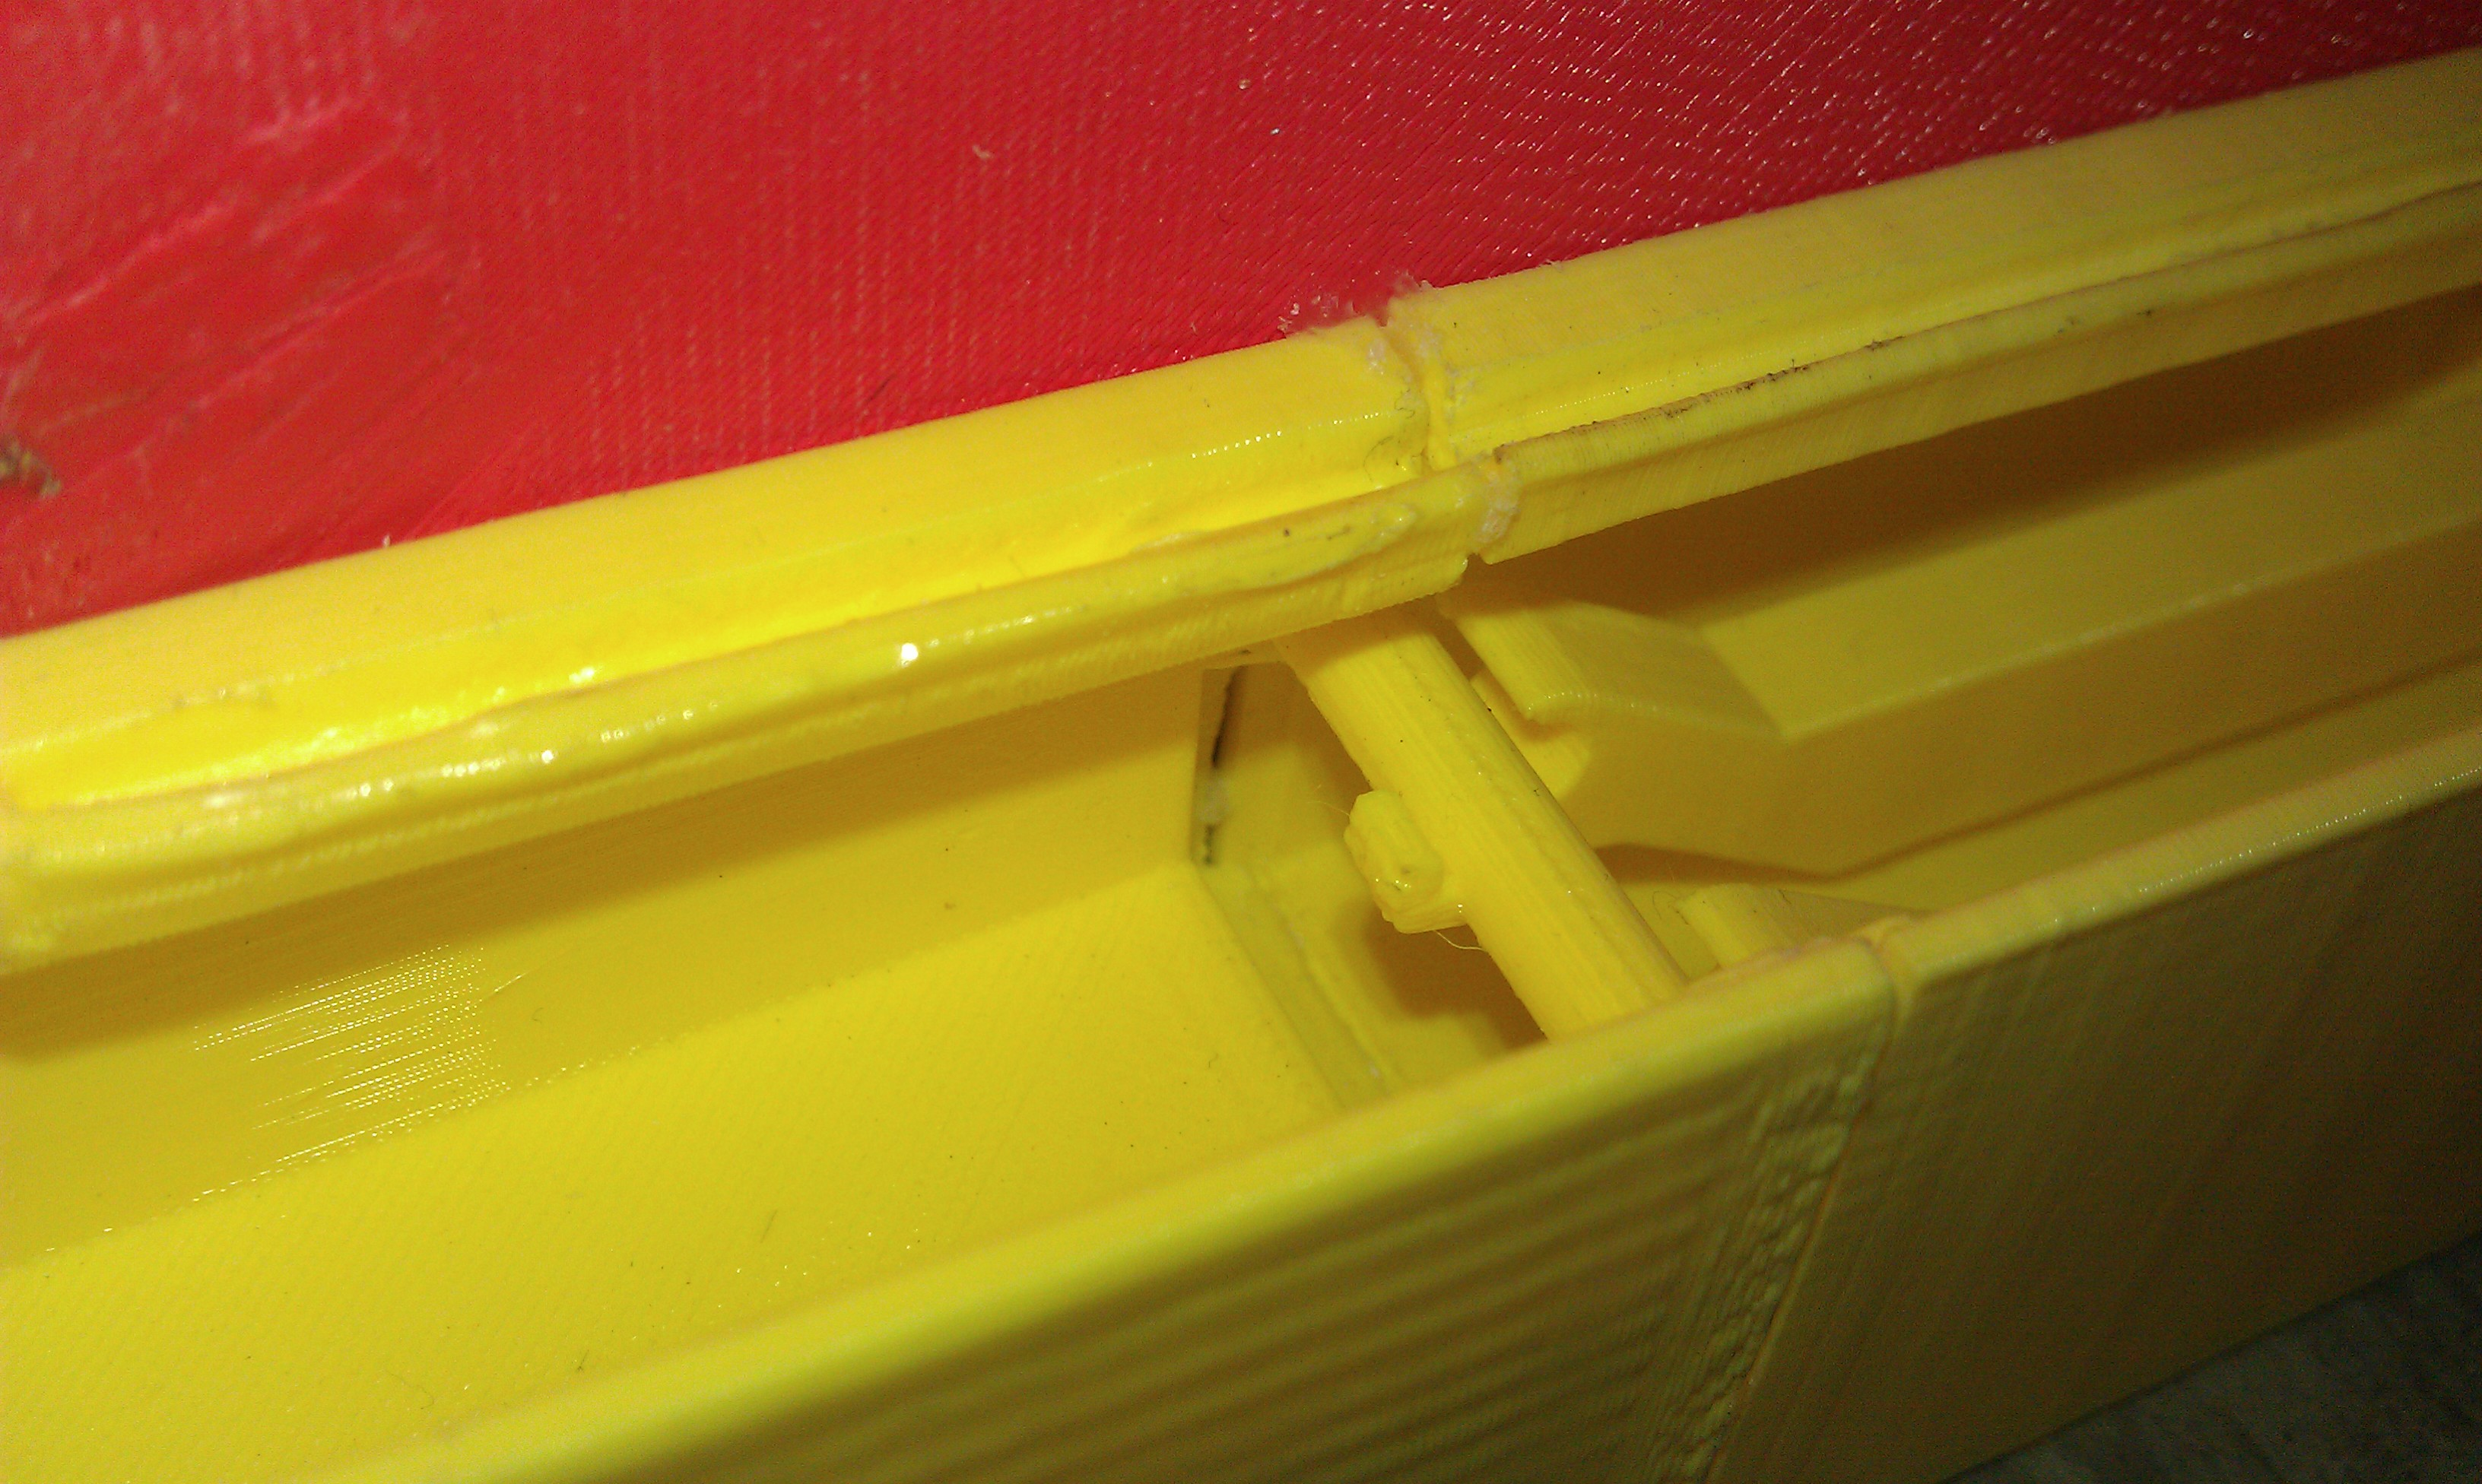
\includegraphics[width=\textwidth,keepaspectratio,clip]{additional-components/keyboard-mechanism.jpg}%
\caption{Keyboard mechanism}
\end{figure}

To access the boards IO ports the case is open in the back.
Here the user will be able to pug in any of the IO devices, and also view the status of the two power net LEDs.
This is also where the user may slide the board in and out of a tight track that hold the board.

The sides are decorated by two side panels.
On the left side the projects name, Barricelli, is written, along with the names of all the group members.
On the right side there is a picture of Nils Aall Barricelli.
Both these side panels were printed laying flat to get a smoother print and higher resolution.
Because this project have a focus on performance, we made these side panels red.
This is because red is well known as the fastest color \cite{red-is-the-fastest-color}.

The board dissipate heat from the power supply, and this heat must get out of the case.
To make the board run cool enough in the case the top of the case is perforated with 42 ventilation holes.

To decorate the case, an NTNU logo was put on the front panel between the user LEDs and the reset button and power LED.

\begin{figure}[H]
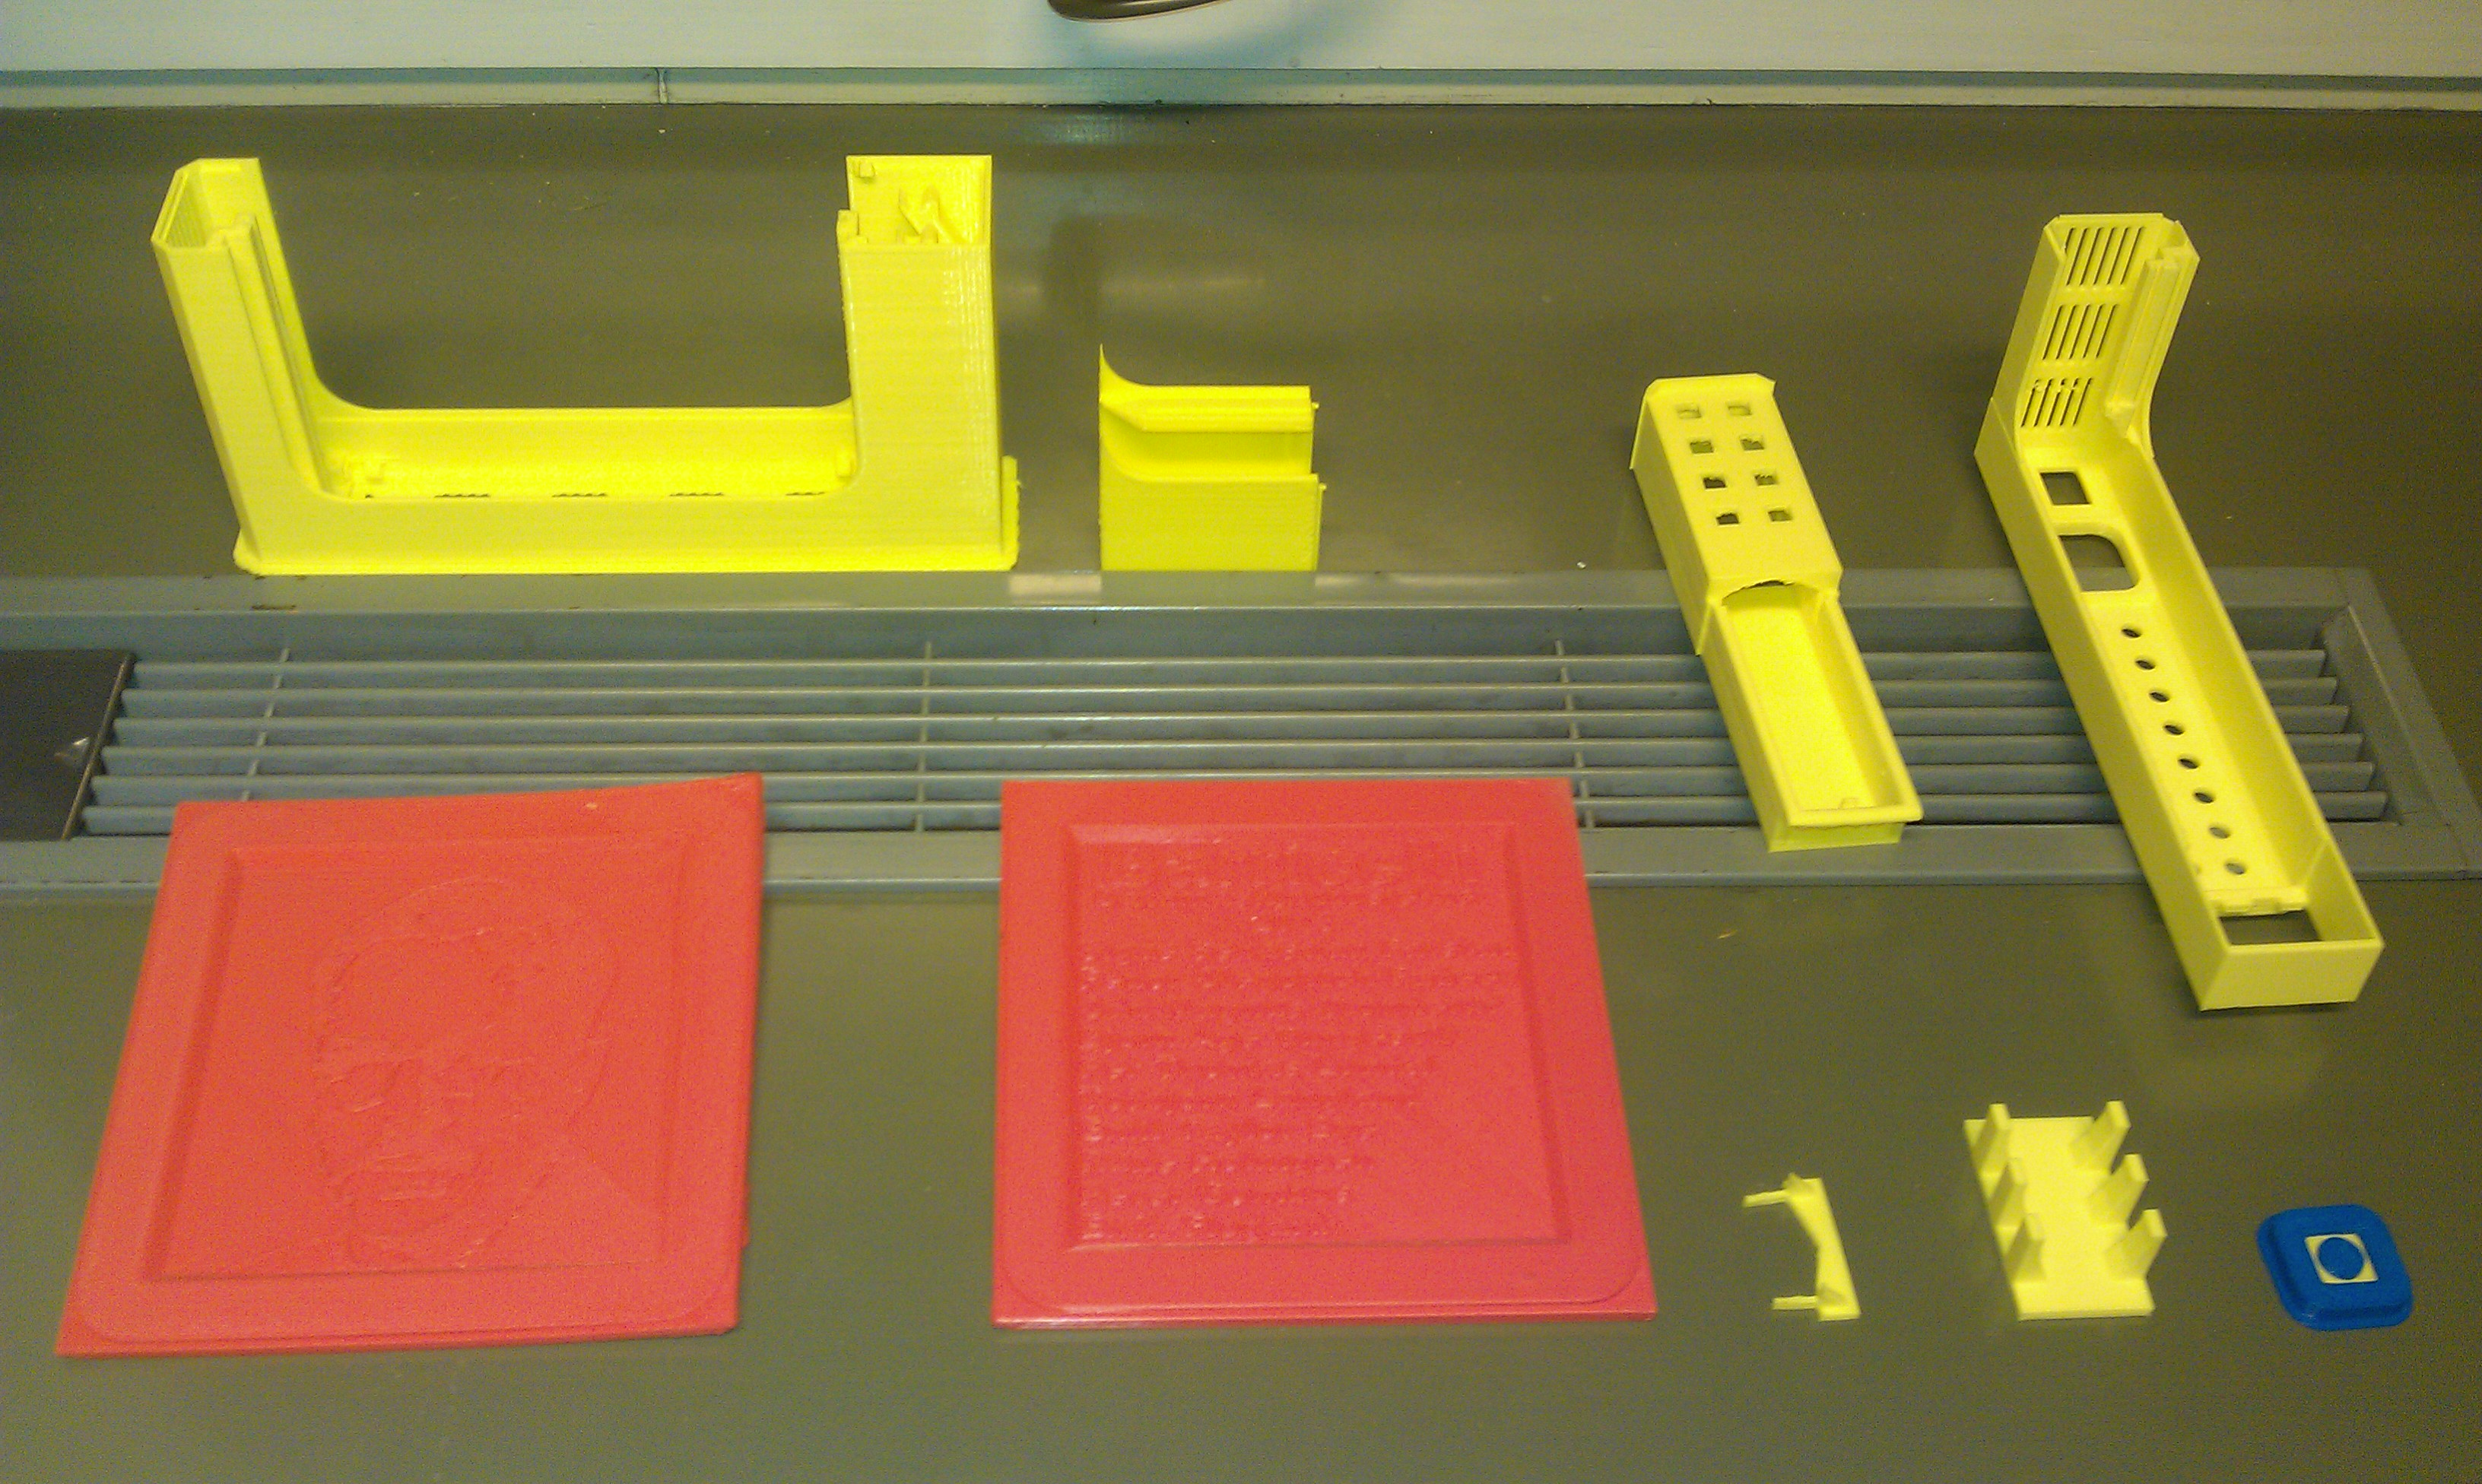
\includegraphics[width=\textwidth,keepaspectratio,clip]{additional-components/case-parts.jpg}%
\caption{Case before assembly. (The two parts of the NTNU logo are already assembled)}
\end{figure}

The case is made up of 10 3D printed parts, 16 user controlled LEDs, a power LED, a reset button, a circuit board with 8 user readable buttons and a whole lot of wiring and resistors.
All of this make a compact case of $20 x 21.5 x 4 cm$ full of useful features.

\subsection{Tools}

\begin{itemize}
    \item MakerBot Replicator 2 Desktop 3D Printer
    \item MakerWare
    \item Google SketchUp
    \item Fine grade sand paper (P240)
    \item A variety of pliers, knifes and pincers
\end{itemize}

\subsection{Problems and workarounds}

\begin{figure}[H]
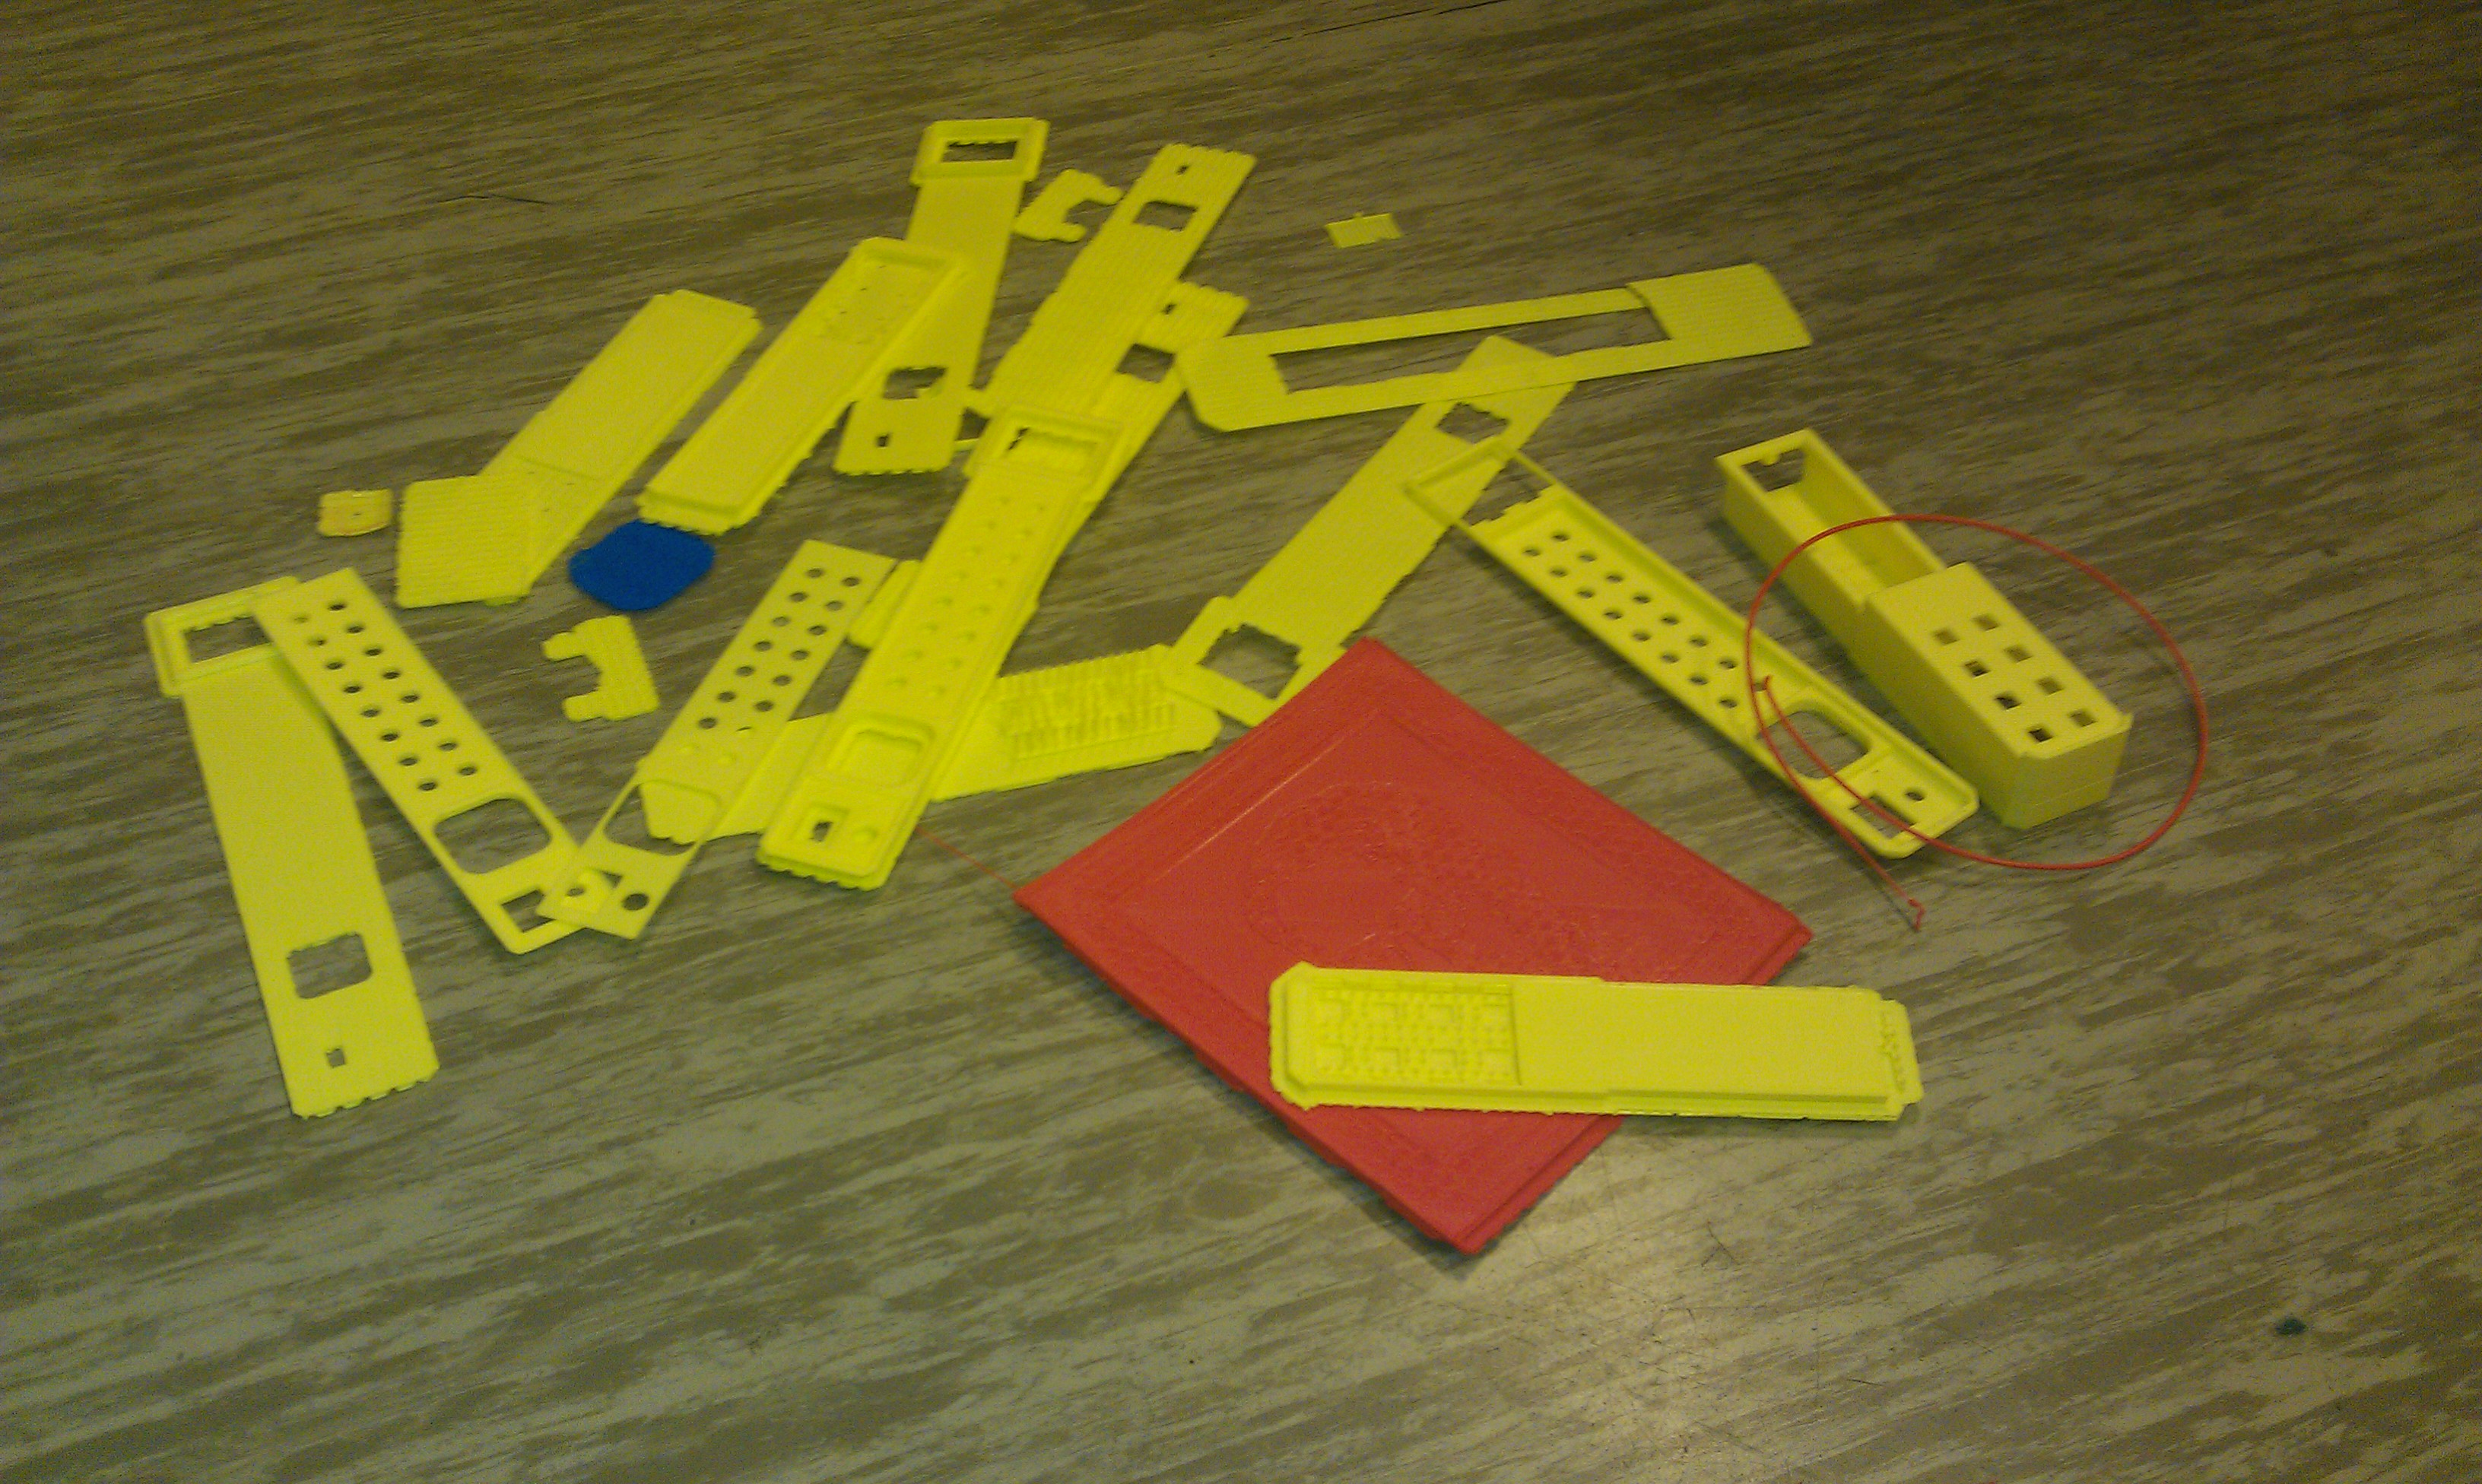
\includegraphics[width=\textwidth,keepaspectratio,clip]{additional-components/some-failed-prints.jpg}%
\caption{Some of the failed prints}
\end{figure}

3D printing is a new technology, and compact desktop 3D printers like the MakerBot 2 is even newer.
As with all other new technology there are problems.
3D printers run into more problems than even normal printers do.
Every time you print a job there is a risk that something will go horribly wrong.
The print may have an error in the compilation, or maybe the PLA plastic filament get tangled or just stop feeding.
In addition, IDI's 3D printer is in horrible shape.
It have got a broken nozzle cooling fan, a partially broken printer head fan and a partially broken PLA filament feeding mechanism replaced with a new 3D printed part.

Because of all these problems, each of the big jobs had to be ran many times before the parts were good enough to be used..
The parts were not all as expected, but with limited time, and jobs that took up towards 20 hours to run they had to do.
The parts that had imperfections were fixed through various hacks.

\subsubsection*{Side panel with Barricelli}
One of the corners had not stuck to the surface during the printing operation.
This may have been caused by the broken nozzle fan.
The result was that one of the corners of the panels was warped by about 5 mm where it was supposed to be flat.
It was however possible to get it almost flat using a heat gun and a hammer.
After that a knife was used to cut away the parts that was supposed to keep the panel in place.
Instead of these parts to keep it in the case, a lot of glue was used.

\subsubsection*{Keyboard tray}
Because of imperfections in the printing process, the keyboard was not able to slide as intended.
This could have been solved by designing it a bit smaller, but the group had almost no experience with 3D printing, and did not know this would be a problem.
It was however solved by sanding it down with fine grade sand paper.

\subsubsection*{Keyboard tray stopper}
The keyboard tray stopper was a bit too wide and tall to actually fit in the case.
This part was small, and could quickly be reprinted.
The problem could also be solved even quicker by cutting of a few millimeters with pliers, so we did that.
The part will not be visible anyway, as it's role is purely functional.

\subsubsection*{Front of the case}
The front of the case was the second larges part of the case.
Because of the complexity of the job, there was a high risk of failure during the job.
After 6 or 7 failed prints the printer had a print that ran about 50\% of the job before failing.
The piece of the part was good enough to be used, and we decided keep that piece, and print the rest as a separate job.
This meant that we had to have an extra glued seem in the completed case, but time was running out so we did it anyway.
The second part of the piece printed fine, and apart from the visible seem it worked out OK.

\subsubsection*{Back of the case}
The back of the case was the largest and most complex part of the case.
To make things worse, it had to be printed in one piece to actually work.
This meant that the printer had to run almost 20 hours non-stop without failing
After many failed prints the printer was abandoned, and we asked a company at NTNU School of Entrepeneurship to borrow their identical, but functioning printer.
Their printer had some minor problems, but the job completed fine at first try.

